\documentclass[12pt]{article}

%packages go here!
\usepackage[hyphens]{url} %Line break of url
\usepackage{anyfontsize}
\usepackage{tikz} %For drawing the cover page's background
\usepackage{graphicx}
\usepackage{titlesec}
\usepackage[a4paper,
	right=2cm,
	left=4.3cm,
	top=2.25cm, bottom=1.25cm]{geometry}
\usepackage[document]{ragged2e} %Left alignment
\usepackage{parskip} %Add an additional line after paragraphs
\usepackage{fancyhdr} %Put numbering on top
\usepackage{enumitem} %List handling
\usepackage{caption} %Caption handling
\usepackage{layout} %Printing out the layout for debugging
\usepackage[backend=biber, style=authoryear-icomp]{biblatex} %Bibliography
\providecommand\phantomsection{} %For putting unnumbered section in toc

%bibliography in latex's path:
\addbibresource{unilink.bib}

%Setting the font
\renewcommand{\rmdefault}{phv} % Arial
\renewcommand{\sfdefault}{phv} % Arial

%Enter parameters here: this is a mark
\newcommand\myauthor{Vo Dang Khoa (D5094; T5616SN)}
\newcommand\mytitle{TESLA, INC}
\newcommand{\subtitle}{}
\newcommand{\rpas}{Report}
\newcommand{\course}{Basics of Business Operations}

\linespread{1.5}

%Redefining maketitle
\renewcommand{\maketitle}{
\thispagestyle{empty}

\begin{center}

\fontsize{16}{19} \selectfont \myauthor

\vspace{20pt}

\MakeUppercase{\fontsize{24}{30} \selectfont \mytitle}

\vspace{5pt}

\fontsize{20}{25} \selectfont \subtitle

\vspace{20pt}

\fontsize{16}{19} \selectfont {\rpas \\ \course}

\vspace{20pt}

\the\year

%Adding the logo
\vspace{100pt}

\includegraphics{logo.jpg}

\end{center}

%Making the cover background
\tikz[remember picture,overlay] \node[inner sep=0pt] at (current page.center){

\includegraphics[width=\paperwidth,height=\paperheight]{coverbg.png}};
\clearpage
}

%Formatting The sections:
\titleformat{\section}
{\bfseries}
{\thesection}
{.17in}
{\MakeUppercase}

%The subsection:
\titleformat{\subsection}
{\bfseries}
{\thesubsection}
{.17in}
{}

%The subsubsection:
\titleformat{\subsubsection}
{\bfseries}
{\thesubsubsection}
{.17in}
{}

%Formatting the paragraphs
%Put new line between paragraphs
\setlength{\parskip}{\baselineskip}
%No indentation
\setlength{\parindent}{0pt}

%Content of the document
\begin{document}
%The cover page
%First we must clear up the margin
\newgeometry{
	right=2cm,
	left=2cm,
	top=4cm,
	bottom=2cm,
	}
{\maketitle}

%Table of content:
\thispagestyle{empty}
{\tableofcontents}

{\clearpage} %% old habits die hard ;-)

%Formatting the margin for the rest of the document
%(If 'restoregeometry' doesn't work then I have no other options":
\newgeometry{
	right=2cm,
	left=4.3cm,
	top=2.25cm,
	bottom=2.5cm,
	}

%Put numbering on top (i.e. the header)
\pagestyle{fancy}
\fancyhf{}
\chead{\thepage}
\renewcommand{\headrulewidth}{0pt} %No line please!

%Formatting lists:
\setlist[itemize]{leftmargin=.6in, nosep} %Vertical spacing of list paragraphs is none

%Caption handling:
\captionsetup[figure]{font=small, position=below}
\captionsetup[table] {font=small, positiona=above}












%The below line was marked!
%===========================================================================================================
%CONTENT GOES HERE!
\section{INTRODUCTION}
This is a report about the basics of Tesla's operation. Additionally, there are more studies on other companies and common business practices as requested by the course's instructor. This report serves mainly for learning purposes so it may not have as much information as papers written by other researchers. References can be found at the end of the text.

\section{BASIC INFORMATION}
This chapter will give some basic information about Tesla, and why this company is interesting for me.

\subsection{Why I chose to investigate Tesla}
This is the company I have heard a lot about for many years and I think it is finally a convenient time to start learning about it. I am also quite interested in alternative energy sources and saving the environment.

\subsection{Basic information}
Tesla currently has 33,000 employees. The company's products are automotive and energy storage. Tesla's headquarters are located in Palo Alto, California. It also has stores located in Canada, Europe, Asia and Australia.

The main market for all of Tesla's car models is the United States. Norway is the largest overseas market for the Model S.

\section{HISTORY}

\subsection{The foundation}
The company was initially founded in 2003 by Martin Eberhard and Marc Tarpenning, although the company also considers Elon Musk, JB Straubel, and Ian Wright as its co-founders.

The founders were influenced to start the company after GM (General Motors) recalled and destroyed all of its EV1 electric cars in 2003. Tesla's early primary goal was to commercialize electric vehicles, starting with a premium sports car aimed at early adopters and then moving as rapidly as possible into more mainstream vehicles, including sedans and affordable compacts for the mass market, serving "as a catalyst to accelerate the day of electric vehicles" (\cite{bry16}).

\subsection{Main business development}
Tesla signed a production contract on July 11, 2005, with Group Lotus to produce "gliders" (complete cars minus powertrain). The contract ran through March 2011, but the two automakers extended the deal to keep the electric Roadster in production through December 2011 with a minimum number of 2,400 units

Musk led Tesla's Series B US\$13 million investment round. Musk co-led the third, US\$40 million round in May 2006. Tesla's third round included investment from prominent entrepreneurs including Google co-founders Sergey Bin and Larry Page. The fourth round in May 2007 added another US\$45 million and brought the total investments to over US\$105 million through private financing.

In October 2008, Musk became CEO and laid off an additional 25\% of Tesla's workforce.

By January 2009, Tesla had raised US\$187 million and delivered 147 cars. Musk had contributed US\$70 million of his own money to the company. Elon Musk owns a 20.8\% stake in the company as of March 2017. The prototype Model S was displayed at a press conference on March 26, 2009. 

In June 2009 Tesla was approved to receive US\$465 million in low-interest-bearing loans from the 2007 US\$8 billion Advanced Technology Vehicles Manufacturing Loan Program by the United States Department of Energy, while Ford got \$5.9 billion, and Nissan got \$1.6 billion. The funding came in 2010, and supported engineering and production of the Model S sedan, as well as the development of commercial powertrain technology. Tesla repaid the loan early and with \$12 million in interest in May 2013, and was the first of the automakers to repay.

On June 29, 2010, Tesla launched its initial public offering (IPO) on NASDAQ. 13,300,000 shares of common stock were issued to the public at a price of US\$17.00 per share. The IPO raised US\$226 million for the company.

\subsection{Most interesting business operations}

In June 2009 Tesla received US\$465 million in loans from the 2007 US\$8 billion Advanced Technology Vehicles Manufacturing Loan Program by the United States Department of Energy, while Ford got \$5.9 billion, and Nissan got \$1.6 billion. But it was the first company to repay the money.

The founders were influenced to start the company after GM (General Motors) recalled and destroyed all of its EV1 electric cars in 2003 (\cite{mu17}).

\section{EXTERNAL ENVIRONMENT}

\subsection{Economic environment}

I will now provide some information on the United States's economy. The source can be found next to the data.

\begin{itemize}
	\item{GDP (in 2016): 18.569 Trillion US\$ (From: World Bank)}
	\item{GDP per capita (in 2016): 57,466.787 US\$ (From: World Bank)}
	\item{Unemployment rate (in August 2017): 4.4\% (From: U.S. Bureau of Labor Statistics)}
	\item{Inflation rate (for 12 months ending in August 2017): 1.9\% (From: http://www.usinflationcalculator.com/inflation/current-inflation-rates/)}
	\item{Trade in 2017 (million US\$): Trade balance: -458,725.2 (a trade deficit); Total exports: 892,621.2; Total imports: 1,351,346.4 (From US' Census Bureau)}
\end{itemize}

Despite having heard of it before, I still find it rather interesting that the biggest economy in the world has a negative balance in trade. Even more interesting is that this deficit is due to consumer products and automobiles, and that the trading partner responsible for this is China. The unemployment is gradually declining, which is a good sign for the economy.

\subsection{Cultural Environment}

I will now discuss about cultural factors of the United States according to (\cite{hoUS}). First of all, there is a high degree of individualism and masculinity in the USA. That important factor plays a crucial role in advertising. Sometimes, showing that you are the best is more important than being actually the best, which is why Elon Musk, current CEO of Tesla decided to initially associate his brand name with the Roadster, a luxurious electric sports car. This car showed to everyone that electric car can be as fast beautiful as any other traditional car.

The US scores below average on Uncertainty Avoidance. As a result, there is a fair degree of acceptance for new ideas and innovative product, something that Tesla also rely on.

However, Americans only score 26 on Long Term Orientation, which means that people don't change their mind easily and will continue to maintain time-honoured traditions and norms. Businesses also prefer to measure their performance on a short-term basis, something that Tesla does have to consider. Still, reality shows that Tesla has been doing well lately on the stock market, which means that investors are confident in the company's long term result.

\subsection{Political Environment}

According to (\cite{ko13}), Tesla wouldn't be a considered successful had it not been for the government's support, particularly from the Advanced Technology Vehicle Manufacturing program and President Obama. After the election of Donald Trump as president, many people worried that Tesla would lose federal support for its business. However, as I mentioned before, the company is still doing fine. \textcite{de16} went as far as saying: "It doesn't make sense for politics to turn against Elon Musk and Tesla", reasoning shutting down his company would result in a big economic loss.

\section{GLOBAL ENVIRONMENT AND INTERNATIONAL TRADE}

The top five trading partners of the US in the current year are China, Canada, Mexico, Japan and Germany (information was received from United States' Census Bureau). Seven out of fifteen trading partners are from Europe.

Tesla opened its first store in Europe in June 2009 in London's Knightsbridge district in the UK, followed by Munich in Germany in September. Tesla's European headquarters are in Amsterdam, the Netherlands.

Norway is the largest overseas market for Tesla's Model S, with 11,802 new units registered through October 2016 thanks to the country's comprehensive incentives for the adoption of pure electric cars. The Parliament of Norway set the goal to reach 50,000 zero emission vehicles by 2018. Among the existing incentives, all-electric cars and utility vans are exempt in Norway from all non-recurring vehicle fees, including purchase taxes, which are extremely high for ordinary cars, and 25\% VAT on purchase, together making electric car purchase price competitive with conventional cars.

\section{BUSINESS ETHICS AND CORPORATE SOCIAL RESPONSIBILITY}

\subsection{Tesla}

Tesla's written code of ethics can be found in (\cite{te10}).

Section "Compliance with Laws, Rules and Regulations" states, "Obeying the law, both in letter and in spirit, is the foundation on which this Company's ethical standards are built. All employees must respect and obey the laws of the cities, states and countries in which we operate. Although not all employees are expected to know the details of these laws, it is important to know enough to determine when to seek advice from supervisors, managers or other appropriate personnel."

Section "Conflicts of Interest" forbids employees from benefiting from things that conflict with the company's interest. An example may be working for another competing company.

Employees are not permitted to use or share confidential information for any purposes except the conduct of their business.

Section "Competition and Fair Dealing" states, "We seek to outperform our competition fairly and honestly. Stealing proprietary information, possessing trade secret information that was obtained without the owner's consent, or inducing such disclosures by past or present employees of other companies is prohibited."

Section "Discrimination and Harassment" says that the company values its diversity as a "tremendous asset". They will not tolerate any illegal discrimination or harassment of any kind.

Many more ethical statements can be found from the aforementioned document. The ones above are just what I find most significant.

According to (\cite{gr17}), Tesla has a corporate social responsibility strategy that relies on the nature of the business. For example, the company's electric automobiles are widely viewed as an answer to the negative impacts of cars that use internal combustion engines. The following are Tesla's stakeholders, arranged according to the company's CSR prioritization:

\begin{itemize}
	\item{Communities (highest responsibility)}
	\item{Customers}
	\item{Employees}
	\item{Investors/Shareholders}
	\item{Governments}
\end{itemize}

About communities, Tesla directly satisfies the concerns of communities as significant stakeholders that determine brand image. One of the interests of this stakeholder group is to ensure that the natural environment is conserved or protected. Tesla's electric automobile products address such interest. For example, communities are satisfied with the fact that these products are environmentally friendly because of zero emissions. Tesla also satisfies communities in terms of this stakeholder group's interest in benefiting from advanced technologies. For example, in 2014, CEO Elon Musk announced that the company would allow other individuals and organizations to use its patents. This corporate social responsibility strategy directly benefits communities interested in using or developing technologies, emphasizing Tesla's mission and vision statements.

For customers, Tesla seeks to improve product quality and pricing. For example, instead of continuing to buy batteries from Panasonic, Tesla plans to manufacture its own batteries to make its electric automobiles more affordable. Also, Tesla continues to expand its network of charging stations.

Tesla satisfies employees' interests through a competitive compensation strategy, as well as HR programs designed to enhance skills development and leadership development.

Tesla's corporate social responsibility strategy addresses investors and shareholders' interests through long-term strategies that aim to transform the automotive market. For example, the company's decision to allow other firms and individuals to use its technology patents is expected to increase market demand for electric vehicles, thereby creating growth opportunities for Tesla automobile sales.

The company satisfies Governments' interest through legal compliance and excellent sustainability, as well as business contribution to economic growth.

Although being the pioneer in the electric car market, Tesla does not just aim to build to build the best electric cars, they want to make the best cars. As evidence from their webpage:

\begin{itemize}
	\item{Quickest Acceleration.}
	\item{Longest Range.}
	\item{The Safest Cars Ever.}
\end{itemize}

Along with that, Tesla also "wanted to prove that people didn't need to compromise to drive electric – that electric vehicles can be better, quicker and more fun to drive than gasoline cars." They "believes the faster the world stops relying on fossil fuels and moves towards a zero-emission future, the better."

\subsection{Google}

Google's ethic codes can be found on (\cite{go17}). "Don't be evil" is the theme emphasize in the company's ethic codes. It is not just about providing their users with unbiased information, but it's also about doing the right thing in generally "following the law, acting honorably, and treating co-workers with courtesy and respect." 

Google expect all of their employees and Board members to follow the Code. Moreover, they expect contractors, consultants and others who work for Google temporarily to follow the Code.

"We hold ourselves to a higher standard in how we treat users", said in the document. Google's responsibility for serving their users include:

\begin{itemize}
	\item{Integrity}
	\item{Usefulness}
	\item{Privacy, Security, and Freedom of Expression}
	\item{Responsiveness: recognize relevant user feedback and do something about it}
	\item{Take action: "Any time you feel our users aren't being well-served, don't be bashful - let someone in the company know about it."}
\end{itemize}

Regarding working relationship, the section "Support each other" includes:

\begin{itemize}
	\item{Equal Opportunity Employment}
	\item{Harassment, Discrimination, and Bullying: Google prohibits discrimination, harassment and bullying in any form – verbal, physical, or visual}
	\item{Drugs and alcohol: Consumption of alcohol is not banned. But any substance abuse is not permitted}
	\item{Safe workplace}
	\item{Dog policy: Google states clearly that it is a dog company}
\end{itemize}

In Google's "About Us" page (\cite{goa17}), they clearly emphasize their social responsibility with headlines like "Meet the researcher using Google Street View to help dementia patients with memory loss", "Studying the sea to make trash less toxic", "The hi-res future of anti pollution tech". We can see they are doing a really good job of marketing based on their social value.

\subsection{Microsoft}

Microsoft's codes of ethics can be found on (\cite{mssbc}) (the document is available in many languages). Some of the standards include:

\begin{itemize} 
	\item{Make good decisions: there are three steps: Pause, Think and Ask}
	\item{Speak up: there is no tolerance for retaliation}
	\item{Trust with out customer: honor privacy and secure data}
	\item{Trust with governments and communities}
	\item{Trust with each other}
	\item{Trust with investors}
\end{itemize}

I have some opinion on Microsoft's statements regarding trust with their customers. Since they have been really infamous for forcing Windows 10 down on Windows 7 and 8 laptops without users' permission (\cite{kle16}).

The company's corporate social responsibility can be found on (\cite{mscsr}). Some of the main things are:

\begin{itemize}
	\item{Empower every person and every organization}
	\item{Environmentally sustainable business practices}
	\item{Increase energy efficiency}
	\item{Minimize the impact of our waste}
	\item{Collaborate with others to tackle pressing environmental challenges}
\end{itemize}

On Microsoft's front webpage (www.microsoft.com), aside from their products you can also find headlines such as "Tackling water scarcity: Microsoft Cloud and Ecolab team up to find solutions". In this article you can find out about how Microsoft's cloud can help businesses reduce water consumption by collecting data, which is a nice example of how technology can change the world.

After reading about all these information on business ethics and corporate social responsibility, I have found out more about how companies and their customers can have a huge impact on societies and the environment. However, I am only convinced that I want to buy an electric car because I know that I can save the planet by doing so. About other things such as business ethics, I cannot trust the company's own guidelines (as mentioned above with Microsoft's case).

\section{MANAGING THE BUSINESS}

\subsection{Investigating Elon Musk}

In this section I will investigate Elon Musk, CEO of SpaceX and Tesla, based on (\cite{ry17}) and (\cite{to17})

Managing a huge business makes personally testing every candidate nearly impossible, but Musk interviewed every candidate himself. Generally, the best candidates get a call with a team manager, and then the best of the best must pass through Elon Musk himself. This fact shows that the entrepreneur puts a lot of effort into hiring the best people and not letting anyone he does not like into the company.

Musk does not require his candidate to have a college or even high school degree. He pointed out that really successful people such as Bill Gates or Steve Jobs all lack college degrees. "If you had a chance to hire them," he has said, "of course, that'd be a good idea."

Talent is important, but Musk also looks for candidates with a positive mindset. "It's very important to like the people you work with," he's said, "otherwise your job is going to be quite miserable."

Elon Musk does not like excessive meetings. Skyler Shuford, who used to work at Musk's SpaceX company, recounted that he once heard a story about Musk telling someone in a meeting, "You haven't said anything. Why are you in here?"

To sum it up, Elon Musk has what I call a "common sense" leadership style. He hires the best people and does not waste time.

\subsection{The mission, vision and strategy of Tesla}

Their goal is simple: "to accelerate the advent of sustainable transport by bringing compelling mass market electric cars to market as soon as possible." Their primary concern is not for the safety of the vehicle, which can be easily replaced, but for the safety of their customers.

Along with that goal comes the strategy. To achieve their first goal, the company initially released an expensive sports car model, take that money to make cheaper cars, then eventually transition to selling average, mass market cars. How they plan to achieve complete safety can be found at (\cite{mu13}).

Tesla's vision is "to create the most compelling car company of the 21st century by driving the world's transition to electric vehicles." They are not interested in just being the best electric car company, they are interested in being the best car company of them all.

\subsection{Tesla's manager}

According to the page at (http://ir.tesla.com/management.cfm), these are the managers of Tesla:

\begin{itemize}
	\item{Elon Musk is the Chairman, Product Architect and CEO. Elon co-founded Tesla and continues to oversee the company's product strategy -- including the design, engineering and manufacturing of more and more affordable electric vehicles for mainstream consumers.}
	\item{JB Straubel is the Chief Technical Officer. As a co-founder of Tesla, JB has overseen the technical and engineering design of the vehicles, focusing on the battery, motor, power electronics, and high-level software sub-systems. Additionally, he evaluates new technology, manages vehicle systems testing, and handles technical interface with key vendors.}
	\item{Deepak Ahuja is the Chief Financial Officer. Deepak brings more than 20 years of global automotive financial experience to the Tesla team. As Chief Financial Officer, Deepak brings invaluable insight of a well-versed industry veteran to help Tesla become a leading automobile company in the world.}

\end{itemize}

\subsection{Recruitment for a managerial position}
Tesla is seeking a person for a position titled "Accessories NA Program Manager". The requirements are:

\begin{itemize}
	\item{BA/BS or the equivalent in experience is required; an MBA is preferred}
	\item{At least 3 years of relevant work experience - Experience launching new vehicle program/products in North America is a plus}
	\item{Experiences/Familiarity in aftermarket vehicle accessories and North America automobile market}
	\item{Excellent communication skills, both verbal and written}
	\item{Strong competency in MS office, Salesforce, and familiarity with Salesforce, Quickbase is a plus}
	\item{Works well under pressure and adapt to changes quickly}
	\item{can manage multiple priorities simultaneously}
	\item{Professional fluency in English/Spanish required; proficiency in other regional languages such as French is a big plus}
	\item{Excellent analytical and problem solving skills}
	\item{Ability to multitask in a fast moving environment and build a strong relationship with other business stakeholders}
\end{itemize}

\subsection{Corporate culture}

According to the webpage at (https://www.hofstede-insights.com/models/organisational-culture/), Organisational Culture is defined as the way in which members of an organisation relate to each other, their work and the outside world in comparison to other organisations. It can either enable or hinder an organisation's strategy.

Tesla's own corporate culture is analyzed in (\cite{me17}). According to the article, Tesla identifies six main features of its organizational culture:

\begin{itemize}
	\item{Move Fast: Speed affects Tesla's competitive advantage. This characteristic of the organizational culture highlights the importance of employees' capability to rapidly respond to trends and changes in the market.}

	\item{Do the Impossible: In developing cutting-edge products, Tesla must ensure that its corporate culture encourages employees to think outside the box.}

	\item{Constantly Innovate: Innovation is at the heart of Tesla Motors, Inc. This feature of the organizational culture focuses on the continuous nature of innovation at the company.}

	\item{Reason from "First Principles": CEO Elon Musk promotes reasoning from first principles, which involves identifying root factors to understand and solve problems.}

	\item{Think Like Owners: Tesla employs its organizational culture as a tool to maintain a mindset supportive of business development. The company wants its workers to think like they own the organization.}

	\item{We are ALL IN: Tesla Motors, Inc.'s organizational culture unifies employees into a team that works to improve the business.}
\end{itemize}

These characteristics of Tesla can be observed directly from the company's CEO Elon Musk himself. As described above, Elon Musk does not waste time, he selects the best people and his "First Principles" thinking is the foundation principle that helped him manage his business at both Tesla and SpaceX.

\section{ORGANISATIONAL STRUCTURES}

\subsection{Tesla's organizational design}

The organization structure of Tesla was discussed in (\cite{me17b}). According to the article, Tesla has an organizational structure that supports continuous business growth. Tesla's organizational structure creates business capabilities that enable strong managerial control despite growing international operations.

Tesla has a functional organizational structure. The following characteristics are the most significant in the company's organizational structure:

\begin{itemize}
	\item{Global hierarchy (most important): This hierarchy involves management teams that control international operations, maintaining strict control over their operations.}
	\item{Global centralization: this organizational structure use one central group to control the entire company.}
	\item{Minimal regional divisions: different divisions are created to implement different strategies and marketing campaign across different countries Tesla's organizational structure has the following divisions mainly used for financial reporting:
	\begin{enumerate}
		\item{United States}
		\item{China}
		\item{Norway}
		\item{Other}
	\end{enumerate}
	}
\end{itemize}

Figure \ref{structpic} is a diagram describing the company's functional hierarchy.

\begin{figure}
	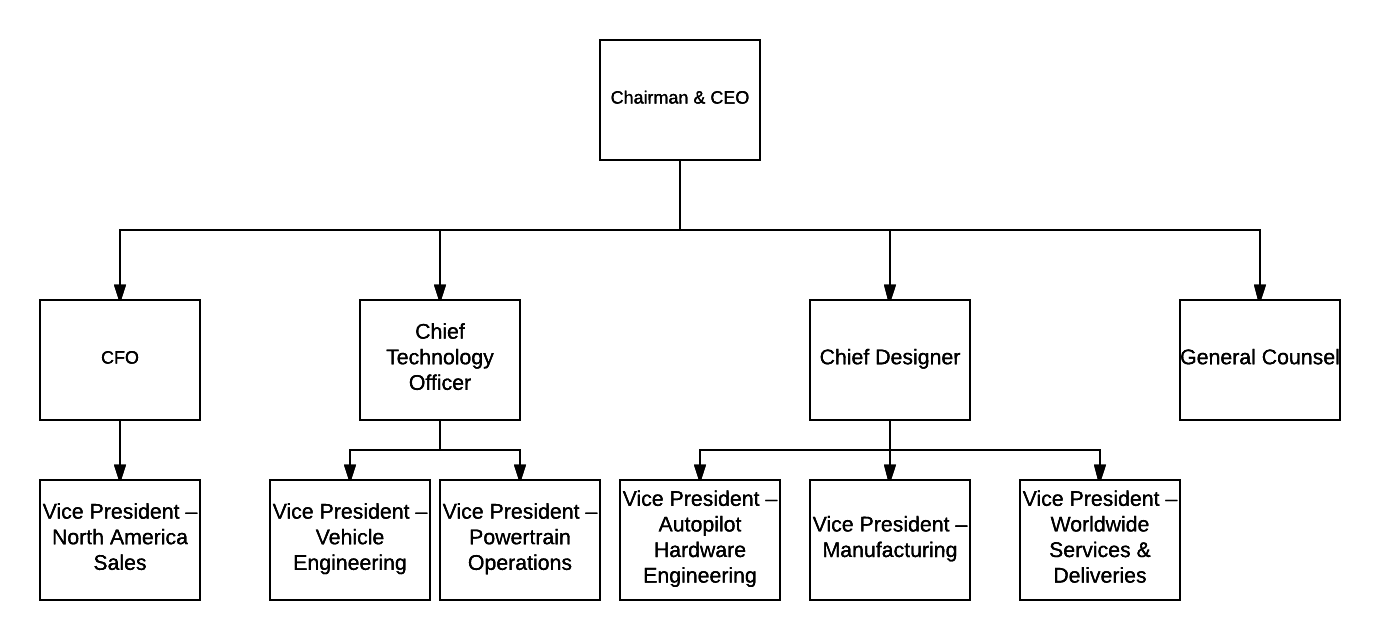
\includegraphics[width=\textwidth]{TeslaStruct.png}
	\caption{Tesla's organizational structure\label{structpic}}
\end{figure}

This organizational structure implies effective control of global operations. However, the lack of decentralization means that it can be hard for overseas branches to flexibly adjust their strategies. The success of overseas offices will rely strictly on the competence of the director board, which can potentially become a disadvantage of Tesla compared to local firms.

\subsection{Departmentalization examples}

Apart from Tesla, another company that adopts \textit{functional departmentalization} is Starbuck Coffee (\cite{me17c}). Starbuck's organizational structure is actually a matrix, which is a mixture of many different grouping methods. For example, the company has an HR department, a finance department and a marketing department with the CEO at the top.

Starbuck also uses \textit{product departmentalization} in its structure. For example, Starbucks has a division for coffee and related products, another division for baked goods, and another division for merchandise like mugs. With each division focusing on its product line, Starbuck can effectively manage its operations.

I unfortunately could not find any example company that uses \textit{process departmentalization} as one of its main division method. However, this method is similar to product departmentalization in a sense that different products involve different processes. However, division based on processes is more specific hence it is not often specified in the main departments.

\section{FINANCING}

\subsection{Concepts}

Financial planning is a generic term which covers a range of different activities concerning costs, revenue, budgetary plans, etc.

The cash-flow forecast resembles the process of preparing a budget. The cash-flow forecast is concerned with the timing of the income and expenditure.

An example of fixed cost can be rent. Likewise an example of variable costs can be the electricity bill of a company making electronic products.

The break-even point is the number of units sold when the company is making no profit,i.e. when the revenue matches the cost.

A balance sheet is a financial statement that summarizes a company's assets, liabilities and shareholders' equity at a specific point in time. These three balance sheet segments give investors an idea as to what the company owns and owes, as well as the amount invested by shareholders. The balance sheet gets its name from the following formula:

\begin{center}
\textit{Assets = Liabilities + Shareholder's Equity}.
\end{center}

Profit \& loss account for the financial year acts as a summary of the trading and profitability of the business over the year as a whole.

What is "equity capital"? When the company starts up, it needs money from different sources and it can come from equity capital like the entrepreneur's own savings, friends, family members and acquaintances. Banks require that around 20\% of the finance provided comes from the entrepreneur before they consider granting a loan.

External liability(external debts) is the amount of money that a company owns to lenders or creditors, as opposed to the money that is owned to shareholders.

\subsection{Real life examples of banks and public financing}

Here are five banks from the United States:

\begin{itemize}
	\item{Bank of America (https://www.bankofamerica.com/): The bank offers business loan with line amount from \$10,000-\$100,000 and as low as 5.75\% interest rate}
	\item{Wells Fargo (https://www.wellsfargo.com/biz/business-credit/loans/term-loan/): Offers unsecured business loan with \$10,000-\$100,000 loan amount and fixed rates from 6.5\% to 23\%}
	\item{Capital One (https://www.capitalone.com): offers loan up to \$3,000,000 with interest rate from 2.9\% to 3.8\%}
	\item{TD Bank(https://www.tdbank.com/): Two options available:
	\begin{itemize}
		\item{Loan (long-term): \$10,000 to \$1,000,000 with fixed interest rate (amount unavailable); standard terms: 3 to 5 years amortization}
		\item{Line of credit (short-term): \$25,000 to \$100,000 with variable interest rate (amount unavailable); standard terms: on demand}
	\end{itemize}}
	\item{HSBC USA (https://www.us.hsbc.com/1/2/home/small-business-banking-solutions/): there are also two options: Lines of Credit and Term Loans}
\end{itemize}

Besides banks providing loans, there is also a company called Y Combinator (http://www.ycombinator.com/) which provide funding (\$120,000) for a large number of startups.

Capital investment refers to money invested in a business with the understanding that the money will be used to purchase fixed assets, rather than used to cover the business's day-to-day operating expenses (from \url{https://www.thebalance.com/capital-investment-2948114}). A capital investor (business angel or capital-investment company) invests money in a target business in return for a share of ownership (typically less than 50 \% of the shares). Capital investors take a significant risk when they make an investment, and therefore they expect a significant return from the investment as compensation (Becoming an entrepreneur in Finland).

Crowdfunding is the practice of funding a project or venture by raising many small amounts of money from a large number of people, typically via the Internet. Examples of online crowdfunding platform are Kickstarter (\url{https://www.kickstarter.com/}) and Indiegog (https://www.indiegogo.com/en).

In Finland, The Centres for Economic Development, Transport and the Environment (ELY centres) can grant subsidies for business ventures and the planning of them, depending on the line of business and the location of the enterprise. Business subsidies or aid are generally discretionary and require that the business's operations are profitable. There is no need to pay back the subsidy or aid.

In my home country (Vietnam), Ho Chi Minh City Startup and Innovation Fund was launched by the city of Saigon to develop its startup ecosystem. Its core focus is on IT, mobile, and agricultural innovators. The fund will prioritize capital to companies working in the city's key industries.

According to Bank of Finland's website at (https://www.suomenpankki.fi/en/bank-of-finland/tasks/), the responsibilities of this European central banks are:

\begin{itemize}
	\item{prepares and implements monetary policy in Finland}
	\item{oversees the stability of the financial system and produces statistics}
	\item{conducts research and economic policy analysis}
	\item{attends to the settlement of interbank payments and investment of its own financial assets}
	\item{maintains the stability and efficiency of payment systems and issues banknotes.}
\end{itemize}

\section{OPERATIONS MANAGEMENT – LOGISTICS AND SUPPLY CHAIN MANAGEMENT}

Information about Tesla's logistics was referenced from (\cite{ho16}), (\cite{om16}) and (\cite{ta14}).

Tesla cars were initially built by Lotus in the UK and flown to customers in the US; later it acquired the former NUMMI factory in Fremont, California that GM and Toyota had recently shuttered. Tesla's plant is less than 18 miles away from company headquarters in Palo Alto. Not only is the Fremont facility a full-service auto plant, but its near-term plans include a supplier park built in the immediate vicinity with a focus on large, heavy parts with extensive variations. Taking integrated manufacturing still further, Tesla is also building an absolutely giant battery factory called "Gigafactory" in nearby Nevada, which will localise battery production from Asia. This plant will take in elemental raw materials like copper and aluminium and produce finished battery packs to feed the car plant. A big gain in Tesla's supply chain will be the Gigafactory. Tesla has partnered with Panasonic at the factory, which Musk has said will reduce battery costs by at least 30\%.

In 2015, the company opened an assembly centre in Tilburg, in the Netherlands for assembly of the Model S from kits shipped from California destined for European customers.

While all battery manufacturing will be under one roof, Tesla will still have to manage the inbound raw materials – much of which will come from far afield – and all the associated logistics and warehousing operations. According to previous company reports, completed battery units will be shipped by rail to the Fremont plant.

Currently the company single-sources most components and tends to work on short-term contracts with suppliers. Expanding production will require new arrangements across its supplier base. Some think Tesla's current approach makes sense. "There are many unique features in a Tesla," said Kumar of Frost \& Sullivan. "Every element in the car has been disrupted and it's a learning process for suppliers and for the industry. These short-term contracts make sense: if a supplier can't cope and creates a roadblock, Tesla can find another who can take up the work. As Tesla ramps up production, a more standard contract will come through."

Not everyone agrees. For one thing, Tesla works primarily on a build-to-order basis, which means bottlenecks in parts supply could be a big headache. Improving supplier relations quickly will be critical, according to Jack Nerad. "If I were trying to establish a car company with staying power, I'd want to develop very deep supplier relationships and be able to depend on the supplier to do some of my R\&D and just be a partner," he said. "It's a different way of operating compared to other car companies."

Tesla has been vocal in their rejection of the traditional franchise-dealer sales model. Preferring instead of selling directly to their consumers, the company argues that the laws prohibiting these transactions are outdated - and the consumer is bearing the brunt of the additional cost. They pioneers in shipping their product digitally. Consumers in the US for instance, can go online to purchase their Tesla and choose amongst a wide array of customisation options. In their Beijing showrooms, Tesla has gone so far as to allow payment through WeChat, China's most popular mobile messaging app. Customers that have paid through this service will also automatically "follow" the company's updates, allowing customers to feel more engaged with the company as they wait for the delivery of their vehicle. However, cutting out the dealership rung of the supply chain has been a challenge - several states in America have filed petitiosn to shut Tesla down. Dealerships in New Jersey, Maryland, Texas and Georgia for instance, have effectively banned Tesla from selling directly to consumers. Despite these restrictions, the company continues to grow even in disputed areas - operating a workaround where customers can view the vehicles in showrooms, but must complete orders online or on the phone and have cars shipped in from elsewhere. Information about ordering Tesla cars can be found at (https://www.tesla.com/support/how-ordering-works).

To try and minimise risk, they keep very little inventory, choosing instead to place most of their customers on a several month long waiting list. Tesla admits that there is little research on the impact of this sales model on consumer demand. So far, there's been inadequate data to support any conclusion regarding the loss of business due to the wait time. However, there are also significant upsides to this practice. By keeping little inventory and essentially producing on demand, Tesla can minimise the amount of capital and risk tied up with storing excess inventory. In addition, the wait encourages additional customisation, a premium that many of their paid customers might not have chosen to pay for if they could immediately drive a stock car off the lot.

Figure \ref{supplypic} describes Tesla's supply chain (including Gigafactory).

\begin{figure}
	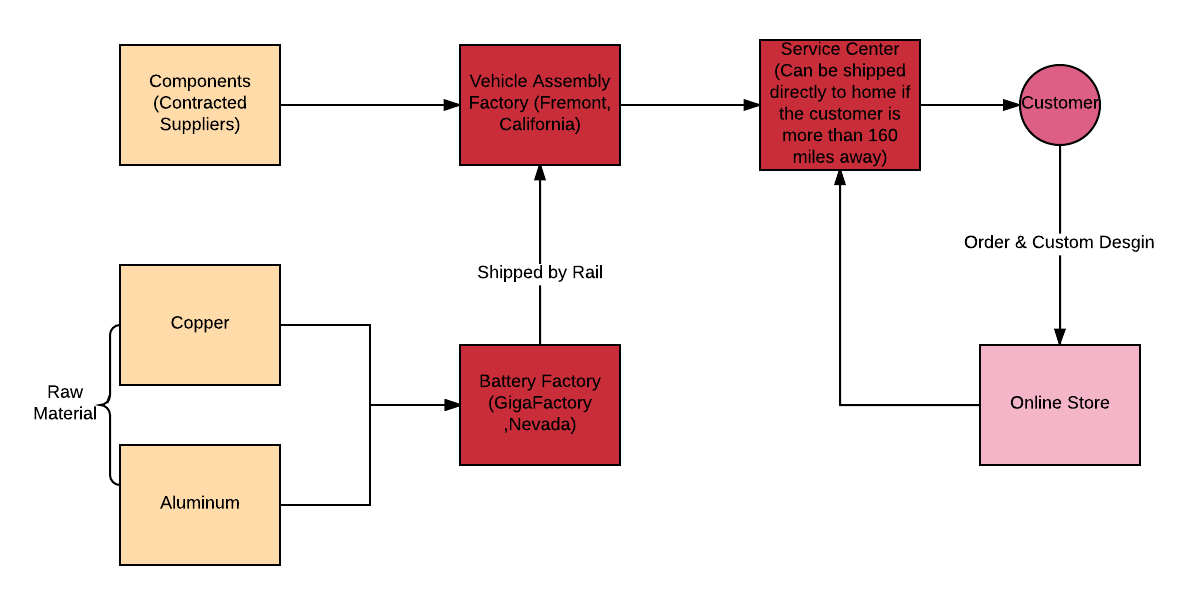
\includegraphics[width=\textwidth]{SupplyChain.png}
	\caption{Tesla's supply chain\label{supplypic}}
\end{figure}

\section{HUMAN RESOURCE MANAGEMENT}

\subsection{Recruitment}


In April, 2010, Tesla Motors announced (\url{https://www.tesla.com/blog/tesla-motors-hires-senior-google-recruiter-world%E2%80%99s-leading-electric-vehicle-man}) that it had hired senior Google staffing strategist Arnnon Geshuri to lead the automaker's rapid recruitment of engineers and other key employees. As vice president of human resources, Geshuri would architect Tesla's recruitment infrastructure and identify candidates for a growing number of job openings.

Geshuri left the company in May 2017 (\cite{ha17}) after eight years in office. He was replaced by Gaby Toledano, who joins the carmaker after a decade on the executive team at Redwood City-based video game publisher Electronic Arts. She will serve as Tesla's chief people officer and report directly to Musk.

\subsection{Career}

Tesla's job openings can easily be found on their website at (\url{https://www.tesla.com/careers/}) and they have a lot of jobs to fill from all over the world. For example, this is the shortened description of a Network support engineer recruitment in Beijing, China:
{\itshape
\begin{itemize}
	\item{Responsibilities:}
	\begin{itemize}
		\item{Respond to day-to-day network support requests from both business customers and IT peers.}
		\item{Areas of responsibility include switches, routers. stateful firewalls, wireless controllers and access points, SSL VPN's, and any other device that provides network services.}
		\item{Monitor network systems and create baselines as part of proactive approach to maintaining high level of service.}
		\item{Participate in on call activities and follow escalation process to provide 24/7 network support.}
		\item{25\% travel required as necessary.}
	\end{itemize}
	\item{Job Experience:}
	\begin{itemize}
		\item{3+ years' experience in Network Engineering is a must. Advanced experience in the following preferred:}
		\item{Experience with troubleshooting protocols including TCP/IP, STP, VRRP, BGP, OSPF and IPSec}
		\item{Experience with scripting and configuration automation using Python or Ansible}
		\item{Demonstrated ability to analyze complex situations and utilize troubleshooting skills, systems and tools, and creative problem solving abilities under pressure.}
		\item{Certifications such as JNCIA or CCNA is required, JNCIP or CCNP is preferred.}
	\end{itemize}
\end{itemize}
}

\subsection{Employer branding}

Employer branding is the firms corporate image or culture created to attract and retain the type of employees the firm is seeking. It is what the company stands for in the public eye. What kind of employer brand does Tesla have? Let's investigate this by looking at what they post on their recruitment advertisements:

{\itshape
"Tesla is committed to hiring and developing top talent from around the world for any given discipline. Based in California, Tesla's workforce spans across four continents. We work to build an inclusive environment in which all people, regardless of gender, race, religion, or background, can come to do their best work.

Our world-class teams operate with a non-conventional philosophy of inter-disciplinary collaboration. Each member of the team is expected to challenge and to be challenged, to create, and to innovate. We're tackling the world's most difficult and important problems—and we wouldn't succeed without our shared passion for making the world a better place."
}

Tesla sees talent and passion as the foremost quality of their employees. They want to create a diverse environment in the workplace. They see problems as challenges and motivate intrapreneuring. On top of all, Tesla distinguish themselves by claiming to "make the world a better place".

\section{IT FOR BUSINESS}

\subsection{IT resources}

The most important resource a company can have is its public website. For example, Tesla sells its car through its website at www.tesla.com. On the site, customers from all around the world can view information about the products available for their country, customize the design and order the cars they want. This business model is both cheap, scalable and easy to manage. The site also has information about job openings so talents from all over the world can join the company. It also contains a database holding data such as stock values and financial reports for investors.

Private network is also a big part in company's management operations. I cannot give any further examples since a good intranet should remain private to the company.

Information system helps in designing and manufacturing process. This is especially true for Tesla since its cars are comparable to sophisticated computer system, as they are almost fully autonomous. According to (\cite{ho16}), Tesla spent around \$1.6 billion in 2015 to prepare for the Model 3 launch, including on people, equipment and automation.

\subsection{Information system}

According to \textit{IGI Global dictionary}, an information service provider is a "provider of a service typified by digital data, for example images and documents". This can be a broad term including any business-related IT service provider such as Tieto Oyj or end-user based Internet Service Provider. Examples for business information service providers include:

\begin{itemize}
	\item{Global Information Service Provider Group (GISP): http://www.gisp-group.com/}
	\item{Salesforce: https://www.salesforce.com/}
	\item{Infosys: https://www.infosys.com/}
	\item{IBM: https://www.ibm.com/}
\end{itemize}

Information systems of Tesla were previously managed by its ex-CIO Jay Vijayan who left in 2016. According to his interview in 2014 (\cite{vi14}), Vijayan said "the IT team built Tesla's entire global systems network and data center infrastructure; software applications for the factory, corporate and retail network; and the necessary information security infrastructure and tools". He stressed in the same interview that building your own IT solution in the age where everyone buys from other comopanies can serve as an advantage in speed, flexibility and seamless integration. Tesla implements IoT in their cars and charging stations to monitor the performance and come up with a plan immediately when problems occur.

Going forward a few years later, the company hired a new CIO to replace Vijayan in 2017. Gary Clark joined the electric car company from Juniper Networks, where oversaw a broad migration to cloud services provided by Amazon Web Services and several SaaS vendors (\cite{bo17}). So with Clark on the board, I expect the company to migrate a large part of its IT operations to the cloud.

\section{Marketing}

\subsection{Case study: Model 3}

For this part I will be looking into Tesla's neweset car model in production: the Tesla Model 3 (Figure \ref{model3pic}). As it will be competing with the Chevrolet Bolt EV, I will use compare the two's number side by side. These are the specifications of the product:

\begin{figure}
	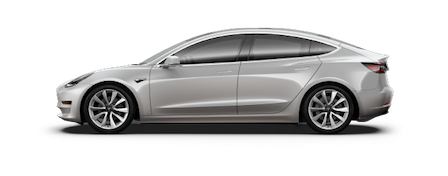
\includegraphics[width=\textwidth]{model_3--side_profile.png}
	\caption{Tesla's Model 3\label{model3pic}}
\end{figure}

\begin{itemize}
	\item{Range: the base model 3 can run for 220 miles before having to recharge, which is slightly less than the Bolt's 238 miles. However, a more expensive Model 3 with a bigger battery can achieve maximum range of 310 miles.}
	\item{Top speed: 130 mph (considerably faster the Bolt's 93 mph)}
	\item{Price: US\$35,000 (a little bit cheaper than the Bolt's US\$37,500)}
	\item{Automatic emergency braking and collisions avoidance}
	\item{15'' touchscreen with onboard map and navigation}
	\item{Wi-Fi and LTE Internet connectivity}
\end{itemize}

As a customer (hypothetically speaking), I deem the Model 3 a superior product to purchase in the future. However, there is another factor to consider: the estimate delivery time. Even if I pre-order right now, I am not expected to receive the car before mid-2018, in contrast to the Chevrolet Bolt which is current out at the moment. In conclusion, I would buy the Bolt simply because I can get my hands on the product in a much shorter time. Besides, it is not that much inferior to the Model 3.

Regarding the instructor's question, the pricing of the car is very competitive. The company's online store makes it very easy to order your car. I have made it clear how to buy the car in previous chapters already, and I will not be repeating that part.

\subsection{Marketing activity}

According to (\cite{schu17}), Tesla does not spend much money promoting their product, only relying on word-of-mouth and free media coverage. This strategy turns out to be working pretty well because of several reasons, in my opinion. First of all, the electric vehicle market is not a saturated one, that's why being a company which sells solely electric cars is enough to set you apart. The second reason is Elon Musk's huge media present and he knows how to take advantage of it to promote his car.

Another thing to mention is their information disclosure. According to (\cite{kro17}), Tesla does not give out certain figures regarding the horsepower and the battery's overall capacity measured in kilowatt-hours. They think that these numbers are confusing and they don't technically matter to the consumer. This is an interesting, unique marketing strategy and it makes a lot of sense to me. In the end, the consumer only care about how fast, how far, and how much. Other technical information should rest with the people involved.

%References: marked!
%---------------------------------------------------------------------------------------------------------------


%These two should always go together
\clearpage

\begingroup 
% NO more line spacing for references
\linespread{1}

% Set spacing between bibliography spacing
\setlength\bibitemsep{\baselineskip}

% NO more hanging indentation for bibliography
\setlength{\bibhang}{0pt}

\section*{REFERENCES}
\phantomsection
\addcontentsline{toc}{section}{REFERENCES}%

\printbibliography[heading=none]
\endgroup















\end{document}
